\documentclass[12pt, a4paper]{article}
\usepackage[utf8]{inputenc}
\usepackage{lscape}   % Make a page in landscape format \begin{landscape}
\usepackage{colortbl} % To color table cells
\usepackage{color} % Able to change textcolor
\usepackage[table]{xcolor}
\usepackage{longtable}
\usepackage{graphicx} % Able to add pictures
\usepackage{parskip}  % Separate paragraphs with a blank line
                      % rather than using indentation
\usepackage{hyperref} % Support for hyperlinks
\usepackage[protrusion=true,expansion=true]{microtype} % Improve justification
\usepackage{subfigure}
\usepackage{hyperref}
\usepackage{caption}
\usepackage{float}
\usepackage{afterpage}
\usepackage{lipsum}
\usepackage{wrapfig}
\usepackage{array}
\usepackage{sidecap}
\usepackage{appendix}
\usepackage{fancyhdr}
\usepackage{changepage}
\usepackage[margin=1.3in]{geometry}
\usepackage{amsmath}
\usepackage{enumitem}


\hypersetup{%
    pdfborder = {0 0 0}
}

\begin{document}
	\begin{titlepage}
\begin{center}

{\Huge \bf Compendium} \\[1.0cm]
{\Huge \bf TDT4242} \\[1.0cm]
{\Large \bf Requirements and Testing} \\[1.0cm]
\vspace{1cm}

{\bf By Marte Løge}


\end{center}
\end{titlepage}
	\tableofcontents
	\clearpage
	\chapter{Introduction}

	This document is a test plan for the ACC system. The ACC system is a 
	tool used for maintenance of software code running in cruise control units in modern 
	automobiles. The test plan consists of a description of all tests planned, in addition 
	an evaluation of consequences and success and failure criteria for each test. 
	The plan is based on our analysis done in exercise one.


	\section{Goal: Control Basis}
	\begin{enumerate}
		\item {\bf Keep the time gap to the car in front automatically}
			\begin{enumerate}[label*=\arabic*.]
				\item The ACC system shall be able to calculate the distance to 
				the preceding vehicle.
					\begin{enumerate}[label*=\arabic*.]
						\item The distance measured by the ACC system should be the same 
						as the physical distance.
					\end{enumerate}
				\item The ACC should be able to maintain the speed according to keep the
				distance to the car in front.
			\end{enumerate}
		\item {\bf Maintain the set speed automatically}
			\begin{enumerate}[label*=\arabic*.]
				\item The ACC system shall be able to determine the speed of the
				subject vehicle.
					\begin{enumerate}[label*=\arabic*.]
						\item The ACC vehicle’s measured speed shall be the same
						as the physical speed.
					\end{enumerate}
				\item The ACC should be able to set the speed according to maintain the 
				set speed.
			\end{enumerate}
		\item {\bf Change automatically between time gap control and set speed control, 
		to which is lower.}
	\end{enumerate}

	\begin{figure}[H]
		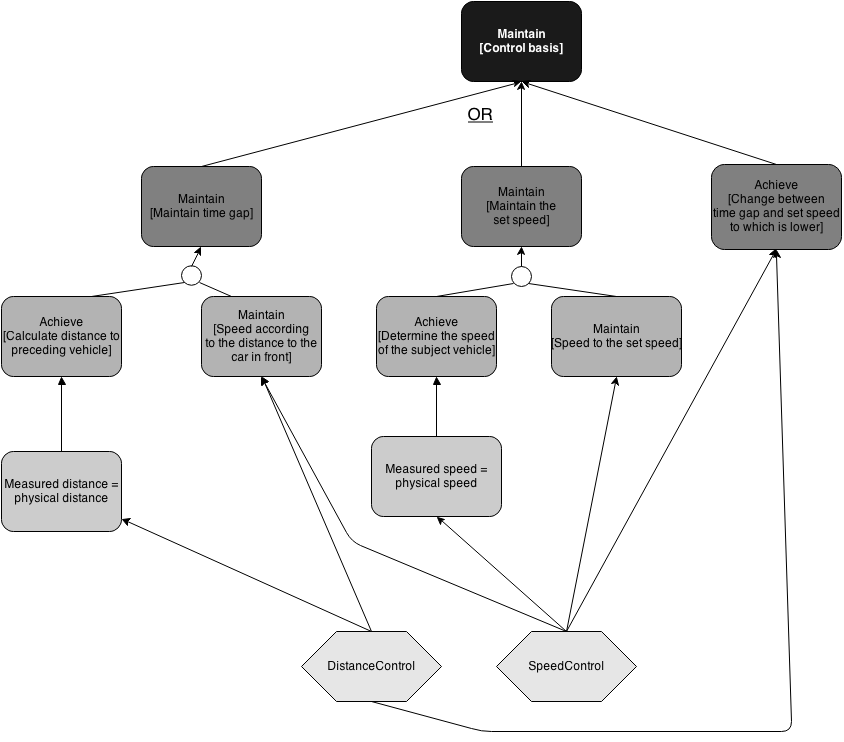
\includegraphics[width=\textwidth]{pics/ControlBasis.png}
	\end{figure}


	\clearpage
	\section{Goal: System States}

	\begin{enumerate}
		\item {\bf ACC system in off state}
			\begin{enumerate}[label*=\arabic*.]
				\item Off state can be set from stand-by state or active state, when 
				the ACC system is turn off, by manually or/and automatically after self test.
				\item Off state can be set from stand-by state or active state automatically
				forced by a failure reaction.
			\end{enumerate}
		\item {\bf ACC system in stand-by state}
			\begin{enumerate}[label*=\arabic*.]
				\item Stand-by state can be reached from off state, manually or/and 
				automatically after self test.
				\item Stand-by state can be reached from active state through a human 
				interface
					\begin{enumerate}[label*=\arabic*.]
						\item Breaking by the driver shall deactivate ACC function at least 
						if the driver initiated brake force demand is higher than the ACC 
						initiated brake force.
						\item For type 1a and 2a systems, the stand-by state may be reached
						from active state when the driver depresses the clutch pedal.
					\end{enumerate}
			\end{enumerate}
		\item {\bf ACC system in active state}
			\begin{enumerate}[label*=\arabic*.]
				\item The active state can only be reached from stand-by state via the human
				interface. 
				\item The active state should switch between time-gap and set speed control
				according to the goal “Control basis”. 
			\end{enumerate}
	\end{enumerate}

	\begin{figure}[H]
		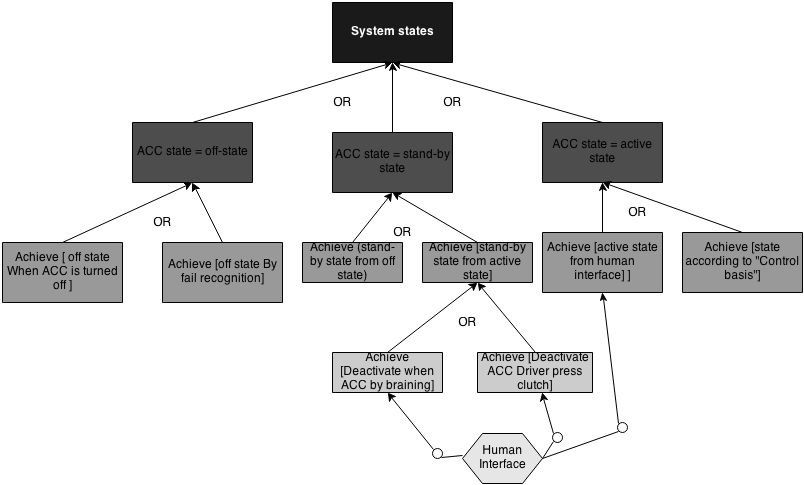
\includegraphics[width=\textwidth]{pics/SystemStates.png}
	\end{figure}
	\clearpage
	\section{Goal: Control Preceding Vehicle}
	
	\begin{enumerate}
		\item {\bf On the roadway, the distance controller should follow the car laying in 
		front in the same lane.}
			\begin{enumerate}[label*=\arabic*.]
				\item If it’s more than one car in front the ACC system should be able 
				to determine which car to follow automatically.
			\end{enumerate}
		\item {\bf ACC distance controller should react on changes in the driving pattern.}
			\begin{enumerate}[label*=\arabic*.]
				\item The car in the front must be in the maximum distance range. 
			\end{enumerate}
	\end{enumerate}	

	\begin{figure}[H]
		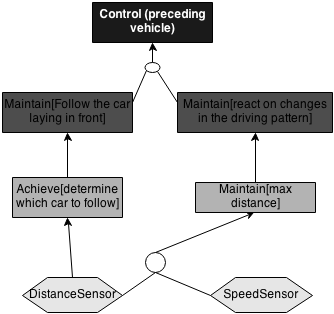
\includegraphics[width=\textwidth]{pics/ControlPrecedingVehicle.png}
	\end{figure}
	
	\clearpage
	\section{Goal: Functional Types}

	\begin{enumerate}
		\item {\bf Type 1a: Manual clutch operation, no active brake control}
		\item {\bf Type 1b: No manual clutch operation, no active brake control}
		\item {\bf Type 2a: Manual clutch operation, active brake control}
			\begin{enumerate}[label*=\arabic*.]
				\item The driver shall be informed clearly and early about a potential 
				conflict between brake and engine idle control. 
			\end{enumerate}
		\item {\bf Type 2b: Active brake control}
	\end{enumerate}

	\begin{figure}[H]
		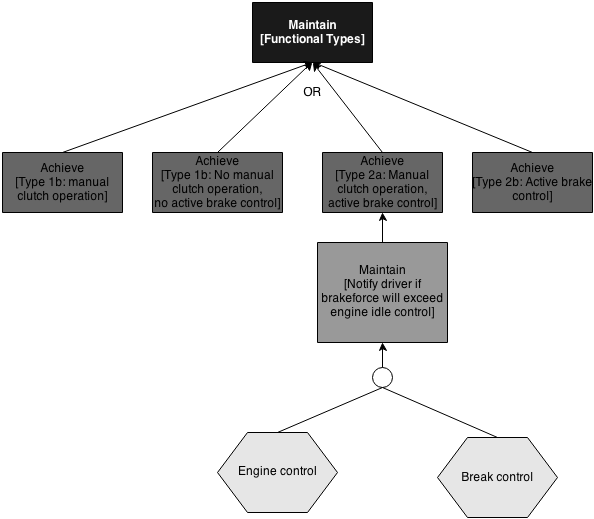
\includegraphics[width=\textwidth]{pics/FunctionalTypes.png}
	\end{figure}

\end{document}

